\documentclass[10pt,a4paper]{article}
\usepackage[margin=20mm]{geometry}
\usepackage{amsmath,amssymb,booktabs,graphicx,xcolor,listings}
\usepackage[hidelinks]{hyperref}
\usepackage{enumitem}
\usepackage[font=small,labelfont=bf]{caption}
\setlength{\parindent}{0pt}
\setlength{\parskip}{5pt}
\setlist[itemize]{nosep,leftmargin=*}
\definecolor{codebg}{RGB}{246,248,250}
\lstset{language=Python,basicstyle=\ttfamily\footnotesize,
  backgroundcolor=\color{codebg},frame=single,rulecolor=\color{black!15},
  breaklines=true,columns=fullflexible,keepspaces=true,
  showstringspaces=false,tabsize=4,aboveskip=6pt,belowskip=6pt}
\newcommand{\TCP}{\mathrm{TCP}}
\newcommand{\R}{\mathbf R}
\newcommand{\p}{\mathbf p}
\newcommand{\q}{\mathbf q}
\title{\vspace{-12mm}EN3563 Robotics Mini Project\\
\large Kinematics and Control of a Simulated GP7\\
\normalsize Upright Pick-and-Place with a Simplified Parallel Gripper}
\author{\small\begin{tabular}{ll}
Member 1 & \textbf{[INDEX NUMBER 1]}\\
Member 2 & \textbf{[INDEX NUMBER 2]}\\
Member 3 & \textbf{[INDEX NUMBER 3]}
\end{tabular}\\
\small Replace the placeholders; remove unused entries.}
\date{Validation: 17 November 2026}

\begin{document}
\maketitle
\vspace{-6mm}

\section{Objective and simulation setup}
A six-degree-of-freedom Yaskawa GP7 was simulated in Gazebo Harmonic using
ROS~2 Jazzy. The objective was to pick a cube from the ground and place it at
the centre of a raised box while preserving its orientation. Robot geometry
and joint axes were obtained from the imported GP7 URDF~\cite{urdf}; the
model was extended with a simplified two-jaw gripper and a grasp tool centre
point (TCP). Dimensions were extracted from the URDF rather than independently
measured from SolidWorks.

\begin{center}
\begin{tabular}{lll}
\toprule
Item & Dimensions (m) & Initial centre / location (m)\\
\midrule
Robot base & Six revolute arm joints & $(0,0,0)$\\
Box A & $0.30\times0.30\times0.20$ & $(0.50,0.30,0.10)$\\
Box B & $0.05\times0.05\times0.05$ & $(0.35,-0.25,0.025)$\\
\bottomrule
\end{tabular}
\end{center}
The target Box B centre is $(0.50,0.30,0.225)$~m because its bottom must rest
on Box A's top surface at $z=0.20$~m. The initial cube point is a fixed selected
reachable point, not a new random sample on every run.

\textbf{Destination deviation:} the task sheet specifies Box A at horizontal
coordinates $(1,1)$~m. That destination is outside the fixed-base GP7's reach.
The implementation therefore retains the selected reachable coordinates above;
this is a documented deviation, not literal compliance with the original
destination. The robot dimensions and base position were not changed.

\section{Coordinate frame assignment and D--H parameters}
Standard Denavit--Hartenberg (D--H) convention is used~\cite{lectures}. Frame $i$ is rigidly
attached to link $i$, and joint $i$ rotates about $z_{i-1}$. Thus $z_0$ is the
joint-1 axis, $z_1$ is the joint-2 axis, and so on through $z_5$ for joint 6.
The $x_i$ axis follows a common normal between adjacent joint axes, and
$y_i=z_i\times x_i$. The following frames are expressed in the base coordinate
system at zero joint angles. The mathematical D--H frames need not equal the
mesh frames in the URDF.

\begin{center}
\begin{tabular}{clccc}
\toprule
Frame & Origin (m) & $x_i$ & $y_i$ & $z_i$\\
\midrule
0 & $(0,0,0.330)$ & $+X$ & $+Y$ & $+Z$\\
1 & $(0.040,0,0.330)$ & $+X$ & $-Z$ & $+Y$\\
2 & $(0.040,0,0.775)$ & $+Z$ & $-X$ & $-Y$\\
3 & $(0.040,0,0.815)$ & $+Z$ & $+Y$ & $-X$\\
4 & $(0.480,0,0.815)$ & $+Z$ & $-X$ & $-Y$\\
5 & $(0.480,0,0.815)$ & $+Z$ & $+Y$ & $-X$\\
6 & $(0.560,0,0.815)$ & $+Z$ & $+Y$ & $-X$\\
\bottomrule
\end{tabular}
\end{center}
The wrist axes intersect at $O_4=O_5$. In this assignment $O_3$ is a different
point on the joint-4 axis, 440~mm from the wrist centre. Thus intersecting wrist
axes do not imply $O_3=O_4=O_5$ for this particular D--H table.
Both $O_0$ and $O_1$ are 330~mm above the floor: $O_0$ is on the fixed
joint-1 axis and $O_1$ is the shoulder origin, displaced 40~mm horizontally.
The 445~mm upright section from $O_1$ to $O_2$ is \emph{link 2}; link 1 is
the rotating base/shoulder body. The two lower origins therefore represent
the base and shoulder, while $O_2$ marks the elbow.

\begin{figure}[htbp]
\centering
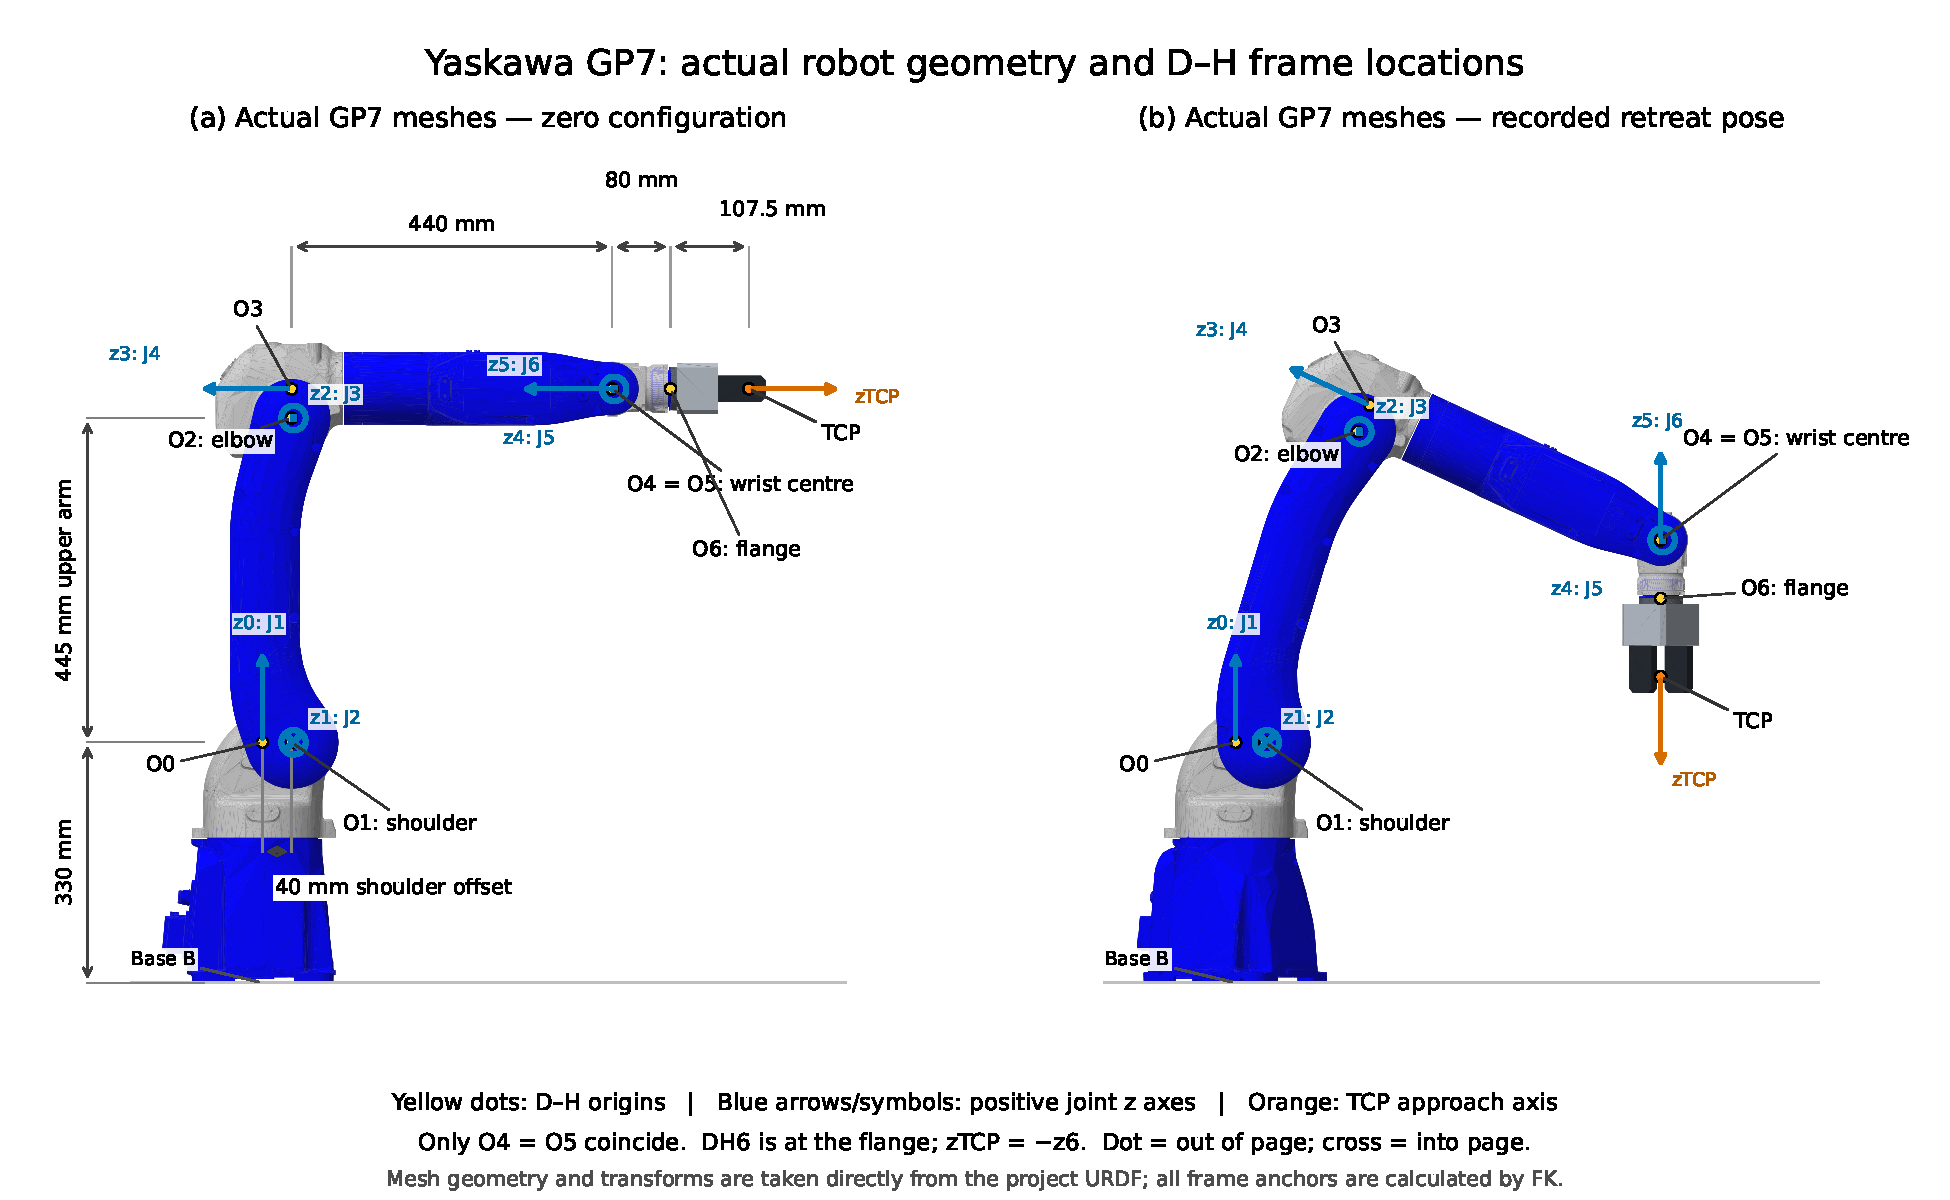
\includegraphics[width=\linewidth]{figures/gp7_robot_frames.pdf}
\caption{The actual GP7 and gripper visual meshes from the simulation URDF,
with FK-calculated D--H origins and positive joint-axis directions.
(a) Zero configuration with the base, shoulder and arm dimensions.
(b) Recorded retreat posture, viewed in its radial plane. Yellow dots mark
origins; blue arrows and dots/crosses identify joint z axes. The coordinate
table defines each complete triad. The flange and TCP are distinct.}
\end{figure}

\begin{center}
\begin{tabular}{clrrrr}
\toprule
$i$ & Joint & $a_i$ (m) & $\alpha_i$ & $d_i$ (m) & $\theta_i$\\
\midrule
1 & S & 0.040 & $-\pi/2$ & 0 & $q_1$\\
2 & L & 0.445 & $\pi$ & 0 & $q_2-\pi/2$\\
3 & U & 0.040 & $-\pi/2$ & 0 & $q_3$\\
4 & R & 0 & $\pi/2$ & $-0.440$ & $q_4$\\
5 & B & 0 & $-\pi/2$ & 0 & $q_5$\\
6 & T & 0 & 0 & $-0.080$ & $q_6$\\
\bottomrule
\end{tabular}
\end{center}
All $q_i$ have the same positive direction as the corresponding URDF joint.
Negative $d_4$ and $d_6$ follow the assigned axis directions and are not
negative physical link lengths. The base height and gripper offset are fixed
transforms outside these six rows.

\section{Forward kinematics}
For each joint,
\begin{equation}
A_i=R_z(\theta_i)T_z(d_i)T_x(a_i)R_x(\alpha_i)
=\begin{bmatrix}
\cos\theta_i&-\sin\theta_i\cos\alpha_i&\sin\theta_i\sin\alpha_i&a_i\cos\theta_i\\
\sin\theta_i&\cos\theta_i\cos\alpha_i&-\cos\theta_i\sin\alpha_i&a_i\sin\theta_i\\
0&\sin\alpha_i&\cos\alpha_i&d_i\\0&0&0&1
\end{bmatrix}.
\end{equation}
Writing $c_i=\cos q_i$ and $s_i=\sin q_i$, substitution gives
\begin{align*}
A_1&=\begin{bmatrix}c_1&0&-s_1&.040c_1\\s_1&0&c_1&.040s_1\\0&-1&0&0\\0&0&0&1\end{bmatrix},&
A_2&=\begin{bmatrix}s_2&-c_2&0&.445s_2\\-c_2&-s_2&0&-.445c_2\\0&0&-1&0\\0&0&0&1\end{bmatrix},\\[3pt]
A_3&=\begin{bmatrix}c_3&0&-s_3&.040c_3\\s_3&0&c_3&.040s_3\\0&-1&0&0\\0&0&0&1\end{bmatrix},&
A_4&=\begin{bmatrix}c_4&0&s_4&0\\s_4&0&-c_4&0\\0&1&0&-.440\\0&0&0&1\end{bmatrix},\\[3pt]
A_5&=\begin{bmatrix}c_5&0&-s_5&0\\s_5&0&c_5&0\\0&-1&0&0\\0&0&0&1\end{bmatrix},&
A_6&=\begin{bmatrix}c_6&-s_6&0&0\\s_6&c_6&0&0\\0&0&1&-.080\\0&0&0&1\end{bmatrix}.
\end{align*}
The fixed transformations and complete chain are
\begin{equation}
{}^BT_0=\begin{bmatrix}1&0&0&0\\0&1&0&0\\0&0&1&.330\\0&0&0&1\end{bmatrix},\qquad
{}^6T_{\TCP}=\begin{bmatrix}1&0&0&0\\0&-1&0&0\\0&0&-1&-.1075\\0&0&0&1\end{bmatrix},
\end{equation}
\begin{equation}
\boxed{{}^BT_{\TCP}(\q)={}^BT_0A_1A_2A_3A_4A_5A_6{}^6T_{\TCP}}
=\begin{bmatrix}\R(\q)&\p(\q)\\\mathbf0^T&1\end{bmatrix}.
\end{equation}
The tool transform equals $R_x(\pi)T_z(0.1075)$: the TCP lies 107.5~mm
along the gripper's positive tool axis, opposite D--H frame 6's $z$ direction.
Here D--H frame 6 is an auxiliary frame \emph{located at the flange}; it is
not identically oriented to the URDF flange/tool frame. The TCP is the
gripper's approach frame, with $z_{\TCP}=-z_6$ when both directions are
expressed in the same reference frame. This explicitly retains the additional
fixed tool transform instead of placing the terminal D--H frame at the TCP.
At $\q=\mathbf0$, matrix multiplication gives
\begin{equation}
{}^BT_{\TCP}(\mathbf0)=
\begin{bmatrix}0&0&1&.6675\\0&-1&0&0\\1&0&0&.815\\0&0&0&1\end{bmatrix}.
\end{equation}
For example, $p_x=.040+.440+.080+.1075=.6675$~m and
$p_z=.330+.445+.040=.815$~m. This agrees with the independently expanded URDF.

In \texttt{kinematics.py}, \texttt{dh\_transform()} constructs each $A_i$,
\texttt{transforms()} multiplies the six matrices, and \texttt{fk()} adds the
TCP transform. The running task uses the equivalent live-URDF chain in
\texttt{urdf\_model.py}; regression tests compare the two models.

\section{Inverse kinematics}
The implemented task solver is \textbf{numerical IK}. To connect it to the
lecture's position/orientation decoupling, the wrist centre for a desired
\emph{TCP} pose is
\begin{equation}
\boxed{{}^{B}\mathbf o_c=\p_d-0.1875\,\R_d
\begin{bmatrix}0\\0\\1\end{bmatrix}}.
\end{equation}
The 0.1875~m offset combines the 80~mm wrist-centre-to-flange distance and the
107.5~mm flange-to-TCP distance along the tool approach direction. It must not
be replaced by the signed D--H value $d_6=-0.080$ when using $\R_d$ for TCP.
The wrist centre depends only on $q_1,q_2,q_3$.

With the present twist signs, the rotational part of $A_4A_5A_6$ is
\begin{equation}
{}^3\R_6=R_z(q_4)R_y(-q_5)R_z(q_6),\qquad
{}^3\R_{6,d}=({}^B\R_3)^T\R_dR_x(\pi).
\end{equation}
Thus the middle angle in a Z--Y--Z decomposition is $-q_5$, not $q_5$; the
fixed TCP rotation must also be removed before using the wrist expression.
These identities explain the lecture connection without claiming that the
demonstrated task uses a closed-form analytical IK solver. The numerical
method below solves position and orientation together under joint limits.

Given a desired TCP transform $T_d=[\R_d,\p_d;\mathbf0^T,1]$, define the
position and orientation residuals
\begin{equation}
\mathbf e_p=\p(\q)-\p_d,\qquad
\mathbf e_R=\operatorname{Log}\!\left(\R_d\R(\q)^T\right)^\vee.
\end{equation}
The rotation logarithm returns a three-component rotation vector and avoids
the ambiguity of subtracting Euler angles. The live-URDF task solves
\begin{equation}
\min_{\q_{\min}\leq\q\leq\q_{\max}}
\left\|\begin{bmatrix}\mathbf e_p\\0.3\mathbf e_R\end{bmatrix}\right\|_2^2.
\end{equation}
The factor 0.3 numerically weights orientation relative to translation.
The first pregrasp solve can retry deterministic alternative seeds; later
waypoints use the preceding solution to encourage a continuous joint branch.
Success requires $\|\mathbf e_p\|<10^{-4}$~m and
$\|\mathbf e_R\|<10^{-3}$~rad. A failed local solve is not a general proof
that a target is unreachable.

The joint bounds in degrees are
\[
\q_{\min}=(-170,-65,-116,-190,-135,-360)^T,\quad
\q_{\max}=(170,145,255,190,135,360)^T.
\]
For the pregrasp target $\p_d=(.35,-.25,.225)^T$~m with
$\R_d=\operatorname{diag}(1,-1,-1)$, one numerical solution is
\[
\q\approx(-35.5377,15.1878,-41.7552,0,-33.0571,35.5377)^T\text{ degrees}.
\]
Substitution into the D--H FK reproduces the desired position and orientation.

\textbf{IK code excerpt} (live-URDF solver, compactly formatted):
\begin{lstlisting}
def residual(q):
    t = self.fk(q)
    return np.r_[t[:3, 3] - target[:3, 3],
        .3 * Rotation.from_matrix(
            target[:3, :3] @ t[:3, :3].T).as_rotvec()]

result = least_squares(residual,
    np.clip(start, self.lower + 1e-8, self.upper - 1e-8),
    bounds=(self.lower, self.upper), max_nfev=250,
    ftol=1e-10, xtol=1e-10, gtol=1e-10)
err = residual(result.x)
if np.linalg.norm(err[:3]) < .0001 and np.linalg.norm(err[3:]) < .0003:
    return result.x
\end{lstlisting}
The separately implemented D--H solver also uses the geometric Jacobian,
$J_{v,i}=z_{i-1}\times(\p-o_{i-1})$, $J_{\omega,i}=z_{i-1}$, with damped
least-squares updates and a bounded-solver fallback. It is an independently
checked mathematical model, while the excerpt above is the solver used by
the demonstrated task.

\section{Trajectory planning and velocity control}
For a Cartesian segment of duration $T$, let $s=t/T$ and
\begin{equation}
\beta(s)=10s^3-15s^4+6s^5,\qquad
\p_d(t)=\p_a+\beta(s)(\p_b-\p_a),\qquad \R_d(t)=\R_{\mathrm{down}}.
\end{equation}
Here $\R_{\mathrm{down}}=\operatorname{diag}(1,-1,-1)$ keeps the tool
pointing downward. The derivatives are
\begin{align}
\dot\p_d(t)&=\frac{30s^2-60s^3+30s^4}{T}(\p_b-\p_a),\\
\ddot\p_d(t)&=\frac{60s-180s^2+120s^3}{T^2}(\p_b-\p_a).
\end{align}
The Cartesian law has zero velocity and acceleration at both ends. Each
segment uses 81 IK waypoints. With a fixed grasp transform, maintaining tool
orientation maintains the carried cube's orientation; the cube's actual
orientation is independently monitored.

\textbf{Trajectory-planning excerpt} (\texttt{URDFModel.cartesian}):
\begin{lstlisting}
points = []
for s in np.linspace(0, 1, samples):
    blend = 10*s**3 - 15*s**4 + 6*s**5
    t = np.eye(4)
    t[:3, :3] = rotation
    t[:3, 3] = start + blend*(finish-start)
    seed = self.ik(t, seed)
    points.append((s*seconds, seed.copy()))
\end{lstlisting}

Joint waypoints are fitted with a clamped cubic spline with zero endpoint
joint velocities. Consequently, the Cartesian reference is quintic, while
the executed joint reference is a cubic spline through the IK waypoints.
Exact Cartesian position and orientation between those waypoints are not
automatically guaranteed by joint interpolation. For the nominal carried
segments, offline checks at 321 points per segment verified position errors
below 0.1~mm and orientation errors below 0.001~rad; this sampled check is not
a proof for every intermediate instant or arbitrary trajectory.
The command supplies positions, velocities and
accelerations to ROS~2's joint trajectory controller~\cite{jtc} so its
interpolation reproduces the cubic intervals. Velocity and acceleration are
continuous within each segment; acceleration continuity across separate
segments and holds is not claimed. In particular, the clamped cubic does not
impose zero endpoint joint accelerations, even though the Cartesian quintic
law has zero endpoint Cartesian accelerations. Position extrema and speed extrema are
checked between waypoints, not only at the knots. Maximum joint speeds are
$(375,315,410,550,550,1000)$ degrees/s.

\textbf{Velocity-command excerpt} (from the spline builder and executor):
\begin{lstlisting}
# controller_trajectory.py
spline = CubicSpline(times, positions, bc_type='clamped')
velocities = spline(times, 1)
accelerations = spline(times, 2)

# pick_place.py: points sent in FollowJointTrajectory
for stamp, q, v, a in zip(times, positions, velocities, accelerations):
    p = JointTrajectoryPoint()
    p.positions = list(map(float, q))
    p.velocities = list(map(float, v))
    p.accelerations = list(map(float, a))
    ns = int(round(stamp*1e9))
    p.time_from_start.sec = ns // 10**9
    p.time_from_start.nanosec = ns % 10**9
    goal.trajectory.points.append(p)
\end{lstlisting}
The controller uses \emph{position} command interfaces with measured position
and velocity feedback. Gazebo's \texttt{gz\_ros2\_control} integration supplies
built-in position-error-to-velocity tracking with configured gain 0.5, a
100~Hz ROS controller rate and a 1~ms physics step~\cite{control}. This is not
a custom velocity PID. The supplied velocity/acceleration fields define the
interpolated position trajectory; they are not separate hardware velocity
commands. Runtime monitoring checks measured speeds and joint positions.
The documented simulated position-interface tracking law is
\begin{equation}
\dot q_{\mathrm{sim},i}=K_p f_c(q_{\mathrm{command},i}-q_{\mathrm{measured},i}),
\qquad K_p=0.5,\quad f_c=100\ \mathrm{Hz}.
\end{equation}
The corresponding project configuration contains
\begin{lstlisting}[language=XML]
<position_proportional_gain>0.5</position_proportional_gain>
\end{lstlisting}

\begin{figure}[htbp]
\centering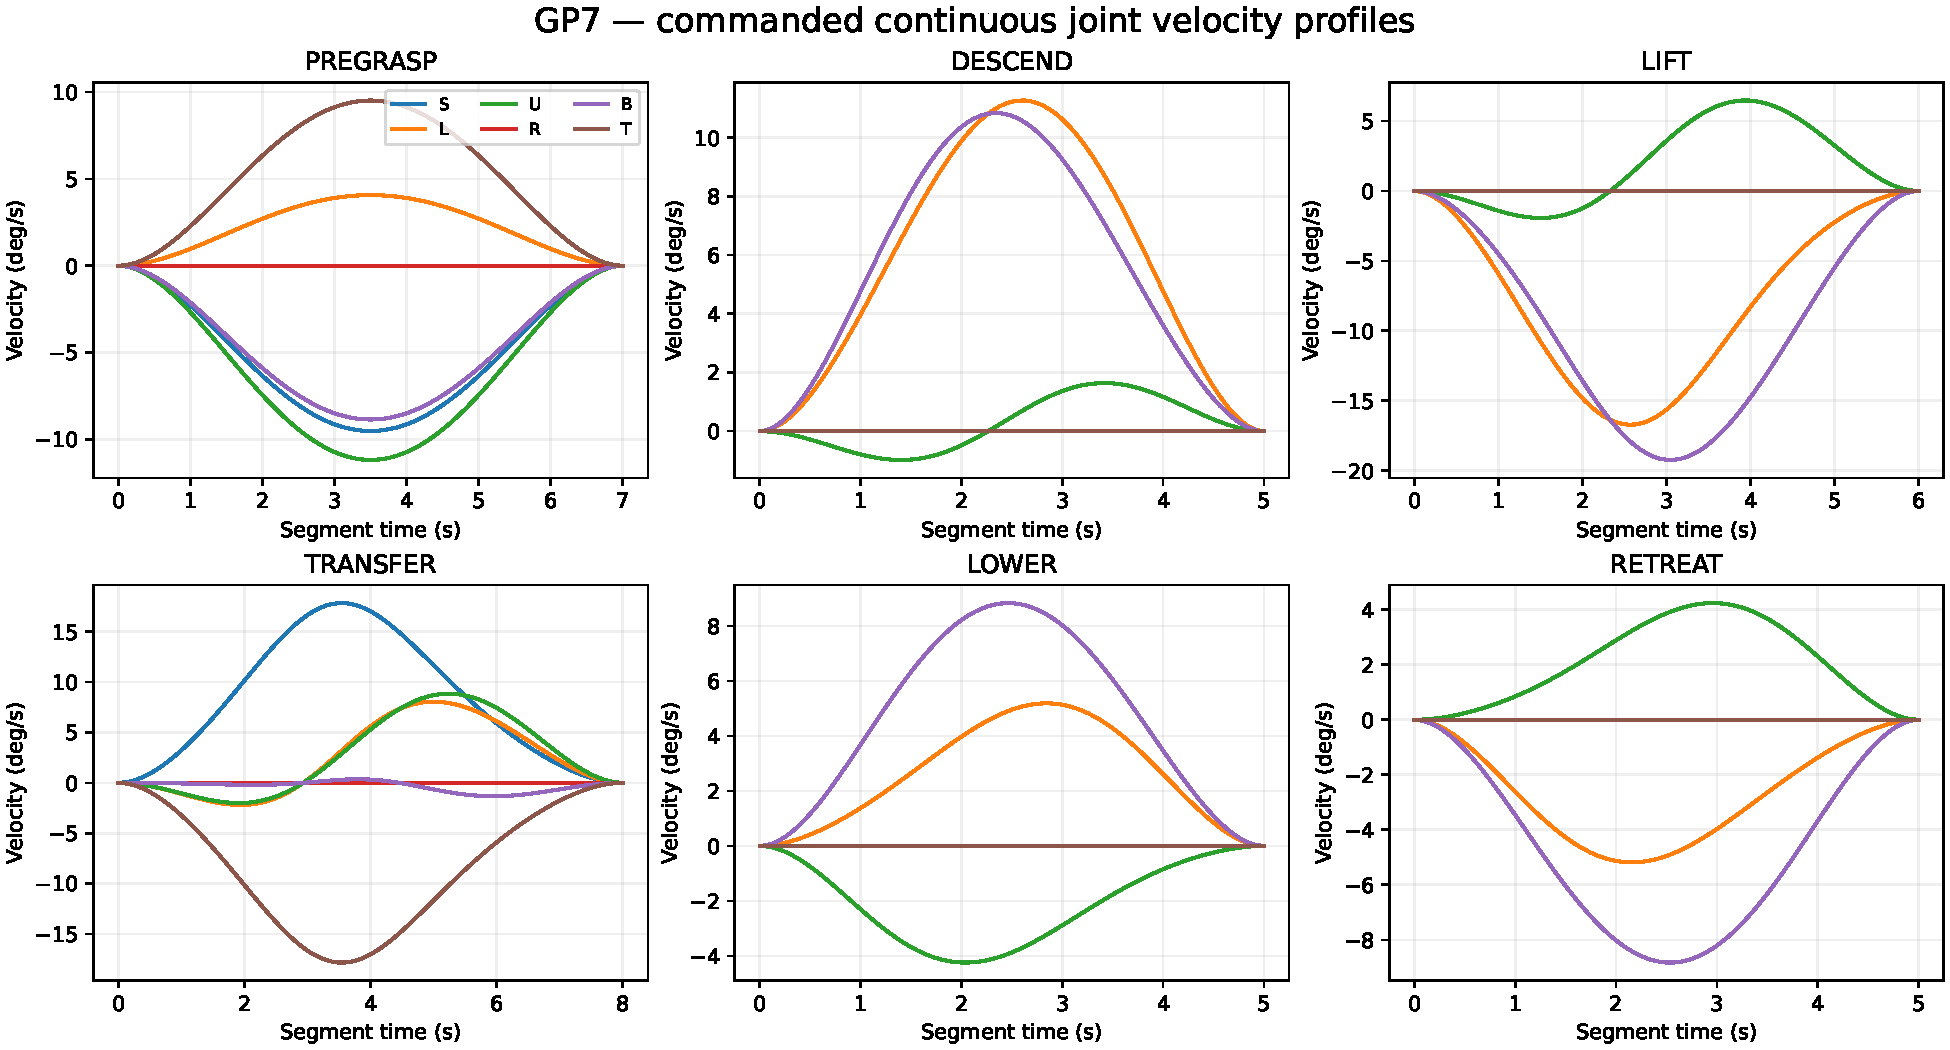
\includegraphics[width=\linewidth]{figures/velocities.pdf}
\caption{Commanded joint velocity profiles for the approach, descent, lift,
transfer, lowering and retreat segments.}
\end{figure}

\section{Implementation process and measured results}
The robot URDF, meshes, gripper and controllers are spawned at the world
origin. FK and IK use the live expanded robot description. The complete
Cartesian path is solved before approach. The arm approaches a point 0.20~m
above the cube, descends, closes the jaws, verifies alignment, lifts to a
0.42~m TCP height, transfers above Box A, lowers to a 0.227~m release height,
releases, verifies settlement and retreats.

Execution advances through
\begin{center}\small
HOME $\to$ PREGRASP $\to$ DESCEND $\to$ CLOSE $\to$ VERIFY\_GRASP\\
$\to$ LIFT $\to$ TRANSFER $\to$ LOWER $\to$ RELEASE\\
$\to$ VERIFY\_PLACE $\to$ RETREAT $\to$ DONE.
\end{center}
Controller acceptance/results, fresh feedback, jaw opening, TCP alignment,
attachment confirmation, measured lift, orientation and stable final placement
are checked. Grasp alignment must be within 2~mm; placement must be within
4~mm and change by no more than 1~mm over the checked 0.5~s interval.
The orientation-change threshold is 0.035~rad ($2.005^\circ$). Monitoring
starts before the approach and continues through retreat.

\textbf{Grasp abstraction:} each jaw leaves 0.5~mm clearance beside the cube.
After alignment is verified, the simulator creates a detachable fixed joint
between gripper and cube. It removes the joint before release. Settlement
then occurs under simulated gravity/contact. This idealized grasp does not
validate friction, grip force or hardware grasp reliability. The cube is not
teleported or moved by a scripted pose animation. Link inertias and motor
effort budgets are simulation approximations.

Fresh headless and GUI runs completed the sequence. The final recorded run
contained 5,071 joint-state samples and 3,062 object-pose samples:
\begin{center}
\begin{tabular}{ll}
\toprule
Measured quantity & Result\\
\midrule
Final cube centre (m) & $(0.500000,0.300000,0.224999)$\\
Position error & $8.6631\times10^{-7}$ m\\
Maximum orientation change & $1.156\times10^{-8}$ degrees\\
Post-retreat drift over checked interval & 0 m\\
Maximum measured joint speed & 0.336 rad/s ($19.2^\circ$/s)\\
Maximum measured speed / its joint limit & 5.43\%\\
Minimum measured joint-position margin & 1.030 rad\\
Task completion time from node start & Approximately 53.54 s\\
\bottomrule
\end{tabular}
\end{center}
These very small errors describe this idealized numerical simulation and
should not be interpreted as physical robot accuracy. The recorded animation
starts during the initial approach; camera/layout changes are visible.

\begin{figure}[htbp]
\centering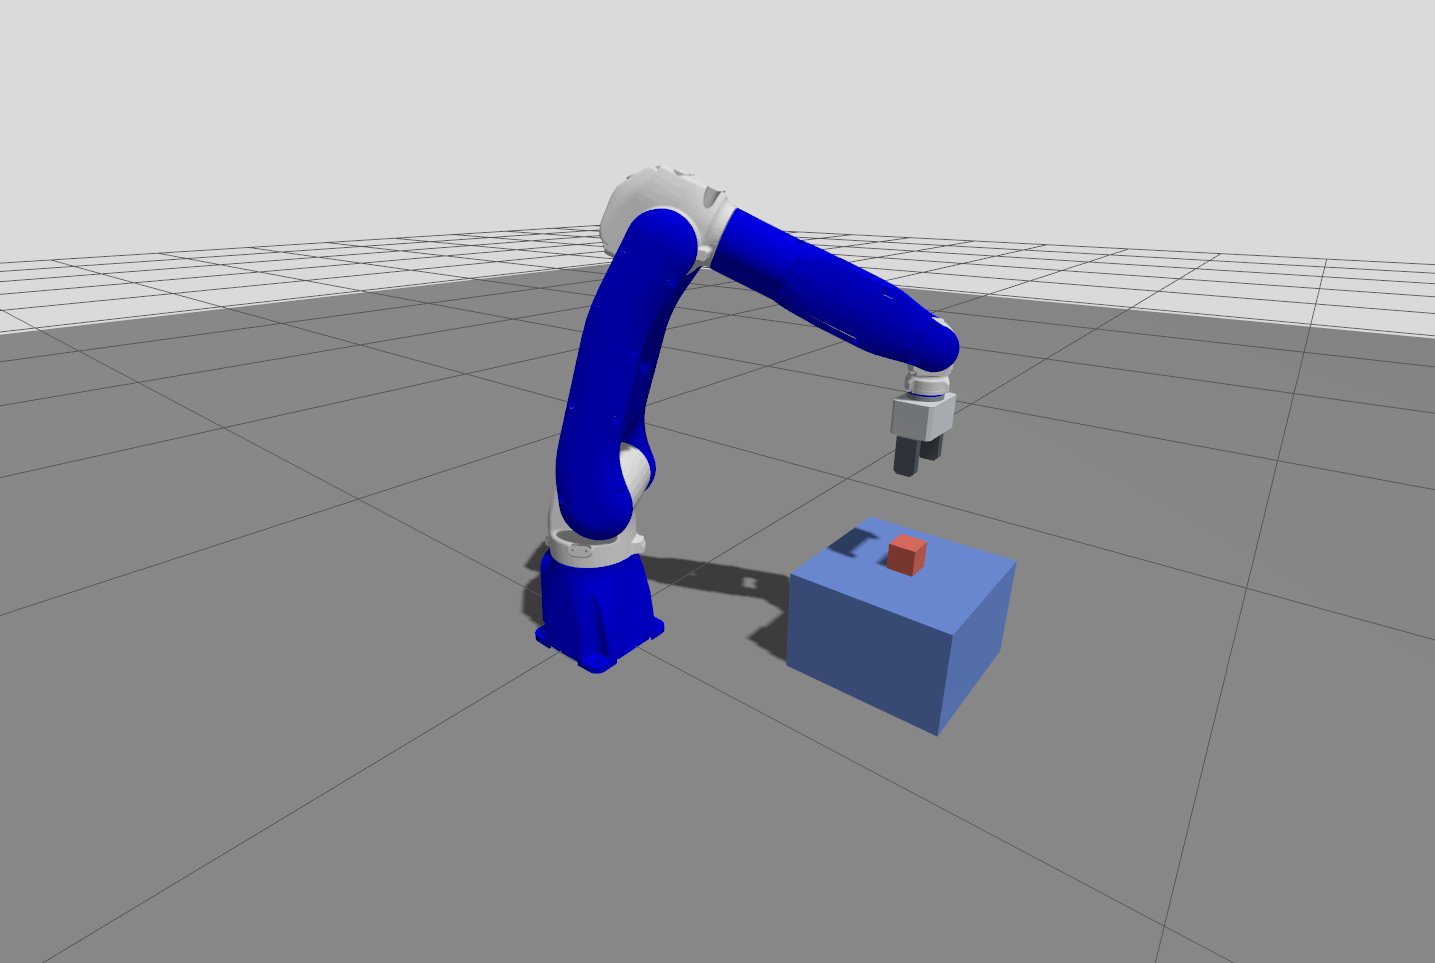
\includegraphics[width=.65\linewidth]{figures/final.png}
\caption{Actual Gazebo view after placement and retreat: the red cube rests
at the centre of Box A's top surface.}
\end{figure}
Sixteen tests pass in both workspace copies. They cover independent D--H/URDF
FK comparisons, Jacobian finite differences, bounded IK, a 180-degree rotation
regression, unreachable-target failure, continuous path interpolation, spline
overshoot/speed checks and state-machine guards. These tests and runs validate
the selected scene; arbitrary targets, global collision avoidance and physical
dynamics are outside the demonstrated scope.

\newpage
\begin{figure}[htbp]
\centering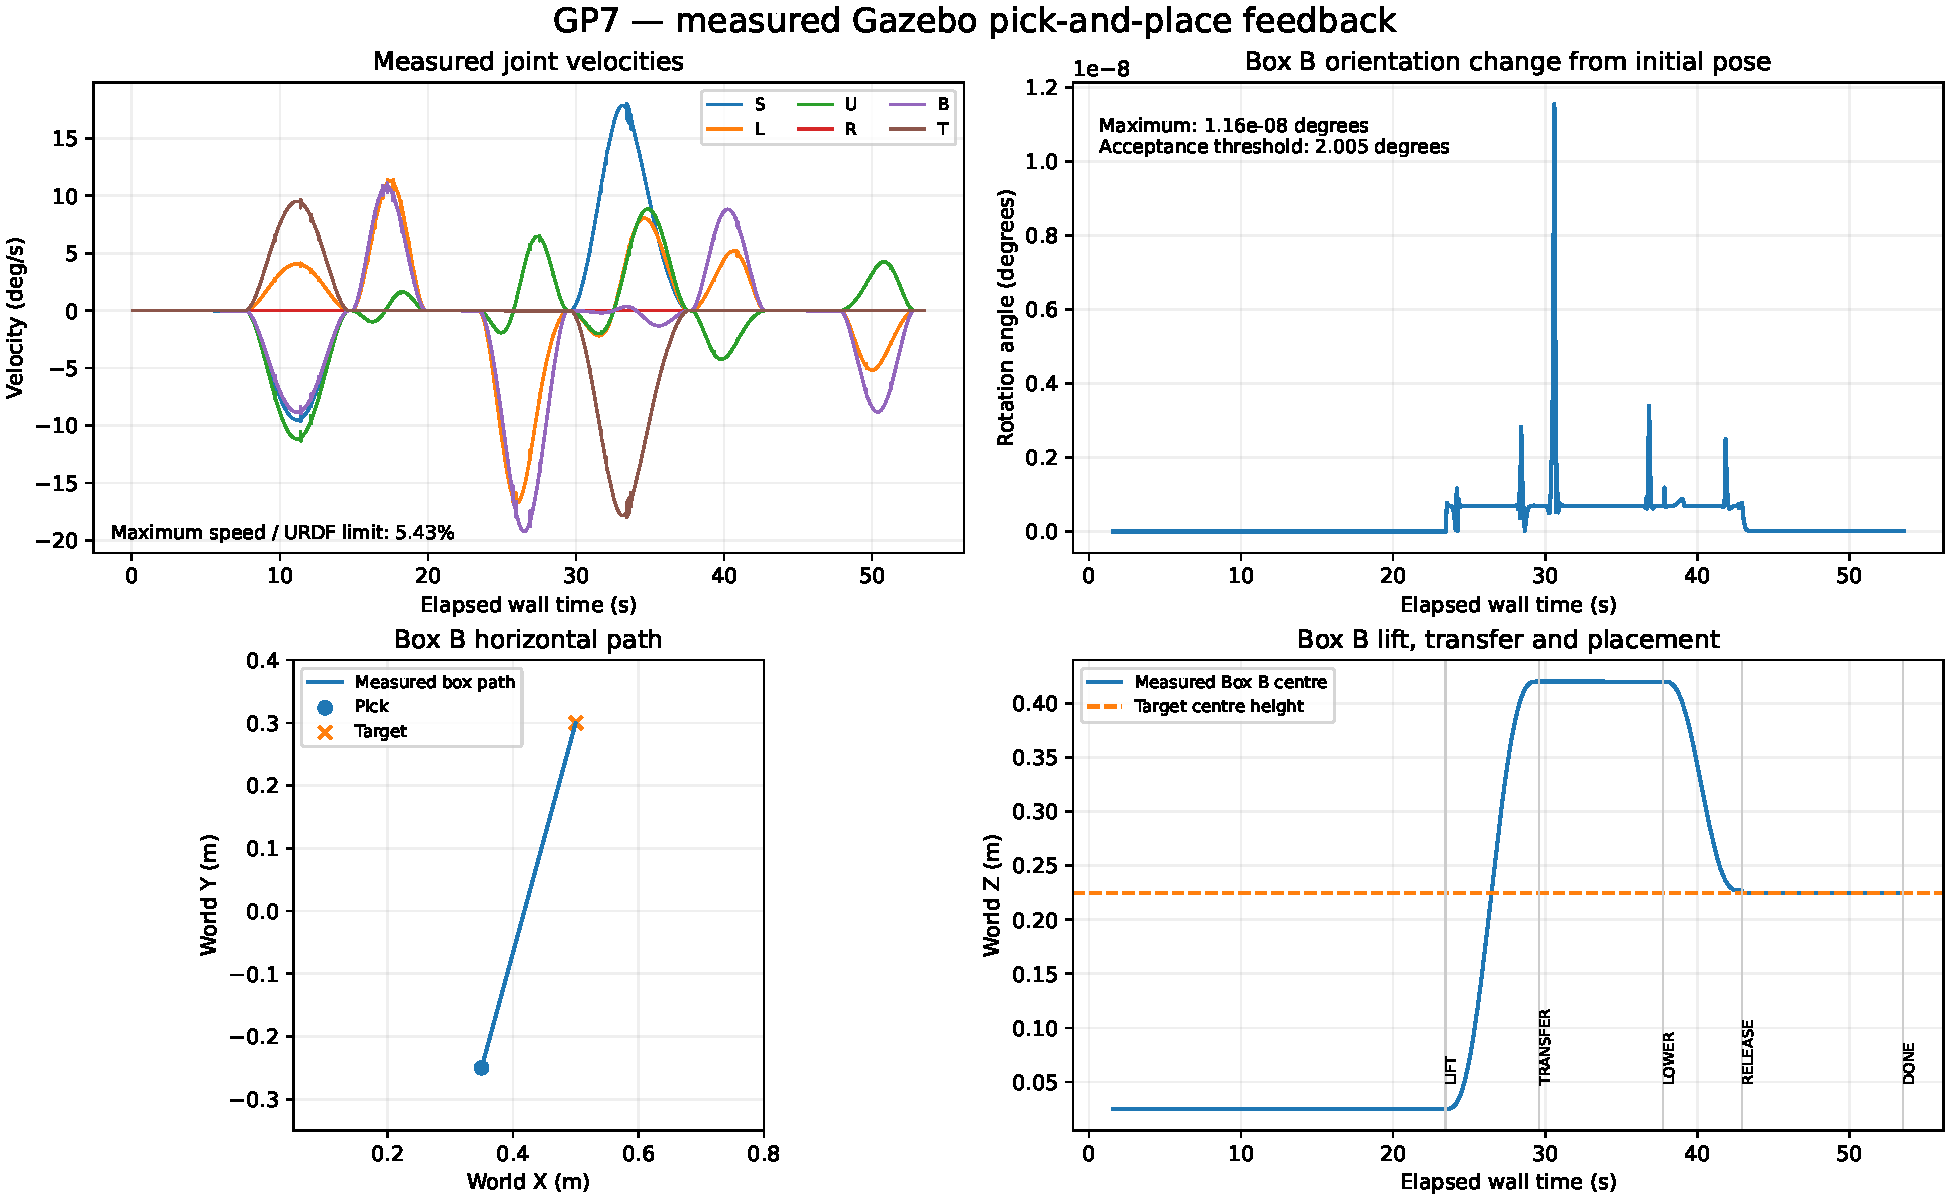
\includegraphics[width=\linewidth]{figures/results.pdf}
\caption{Measured joint velocities, object orientation change, horizontal
transport path and cube height from the recorded simulation run.}
\end{figure}

\clearpage
\section{Conclusion and submission artifacts}
The six-axis simulated GP7 picks and places the cube at the selected reachable
destination while preserving its measured orientation and remaining within
joint limits. The report provides a consistent frame assignment, D--H table,
FK matrices, numerical IK equations and actual planning/control excerpts.
The destination deviation and idealized grasp must be retained when describing
the results.

Submit this report after replacing the member-index placeholders, together
with the recorded simulation video \texttt{gp7\_verified\_demo\_720p.mp4}.
The project includes measured CSVs, plots, logs and \texttt{result.json}.
If the optional code repository is submitted, add its actual URL here:
\textbf{[OPTIONAL REPOSITORY URL]}.

\begin{thebibliography}{9}
\bibitem{lectures} P. Jayasekara, \emph{EN3563 Robotics course notes},
Lectures 6--9 and 11--12, Department of Electronic and Telecommunication
Engineering, University of Moratuwa. Supplied lecture PDFs.
\bibitem{urdf} Maarten de Vries / fizyr, \emph{Yaskawa GP7 support}, Apache-2.0,
imported geometry and meshes, commit
\texttt{47ebe48f9177c79ab0417625ed121c3edb46234a}.
\url{https://github.com/fizyr/yaskawa_gp7_support}.
\bibitem{jtc} ROS 2 Controllers, \emph{Joint Trajectory Controller:
Trajectory Representation, Jazzy}.
\url{https://control.ros.org/jazzy/doc/ros2_controllers/joint_trajectory_controller/doc/trajectory.html}.
\bibitem{control} ROS 2 Control, \emph{gz\_ros2\_control, Jazzy}.
\url{https://control.ros.org/jazzy/doc/gz_ros2_control/doc/index.html}.
\end{thebibliography}
\end{document}
